% Chapter 1

\chapter{Introducción general} % Main chapter title

\label{Chapter1} % For referencing the chapter elsewhere, use \ref{Chapter1} 
\label{IntroGeneral}

%----------------------------------------------------------------------------------------

% Define some commands to keep the formatting separated from the content 
\newcommand{\keyword}[1]{\textbf{#1}}
\newcommand{\tabhead}[1]{\textbf{#1}}
\newcommand{\code}[1]{\texttt{#1}}
\newcommand{\file}[1]{\texttt{\bfseries#1}}
\newcommand{\option}[1]{\texttt{\itshape#1}}
\newcommand{\grados}{$^{\circ}$}

%----------------------------------------------------------------------------------------

En este capítulo se presenta una breve introducción sobre el acopio de cereales y la necesidad de monitorizarlo, soluciones existentes, motivos por los cuales se seleccionó el tema, objetivos y alcance del trabajo. 
%----------------------------------------------------------------------------------------
\section{Descripción de la problemática}

\subsection{Plantas de acopio}

Las plantas de acopio de cereales son depósitos donde se almacenan las semillas luego de ser cosechadas en el campo, a la espera de ser despachadas a su destino final. Estas plantas están compuestas por uno o más silos como puede observarse en la figura \ref{fig:planta}

\begin{figure}[htbp]
	\centering
	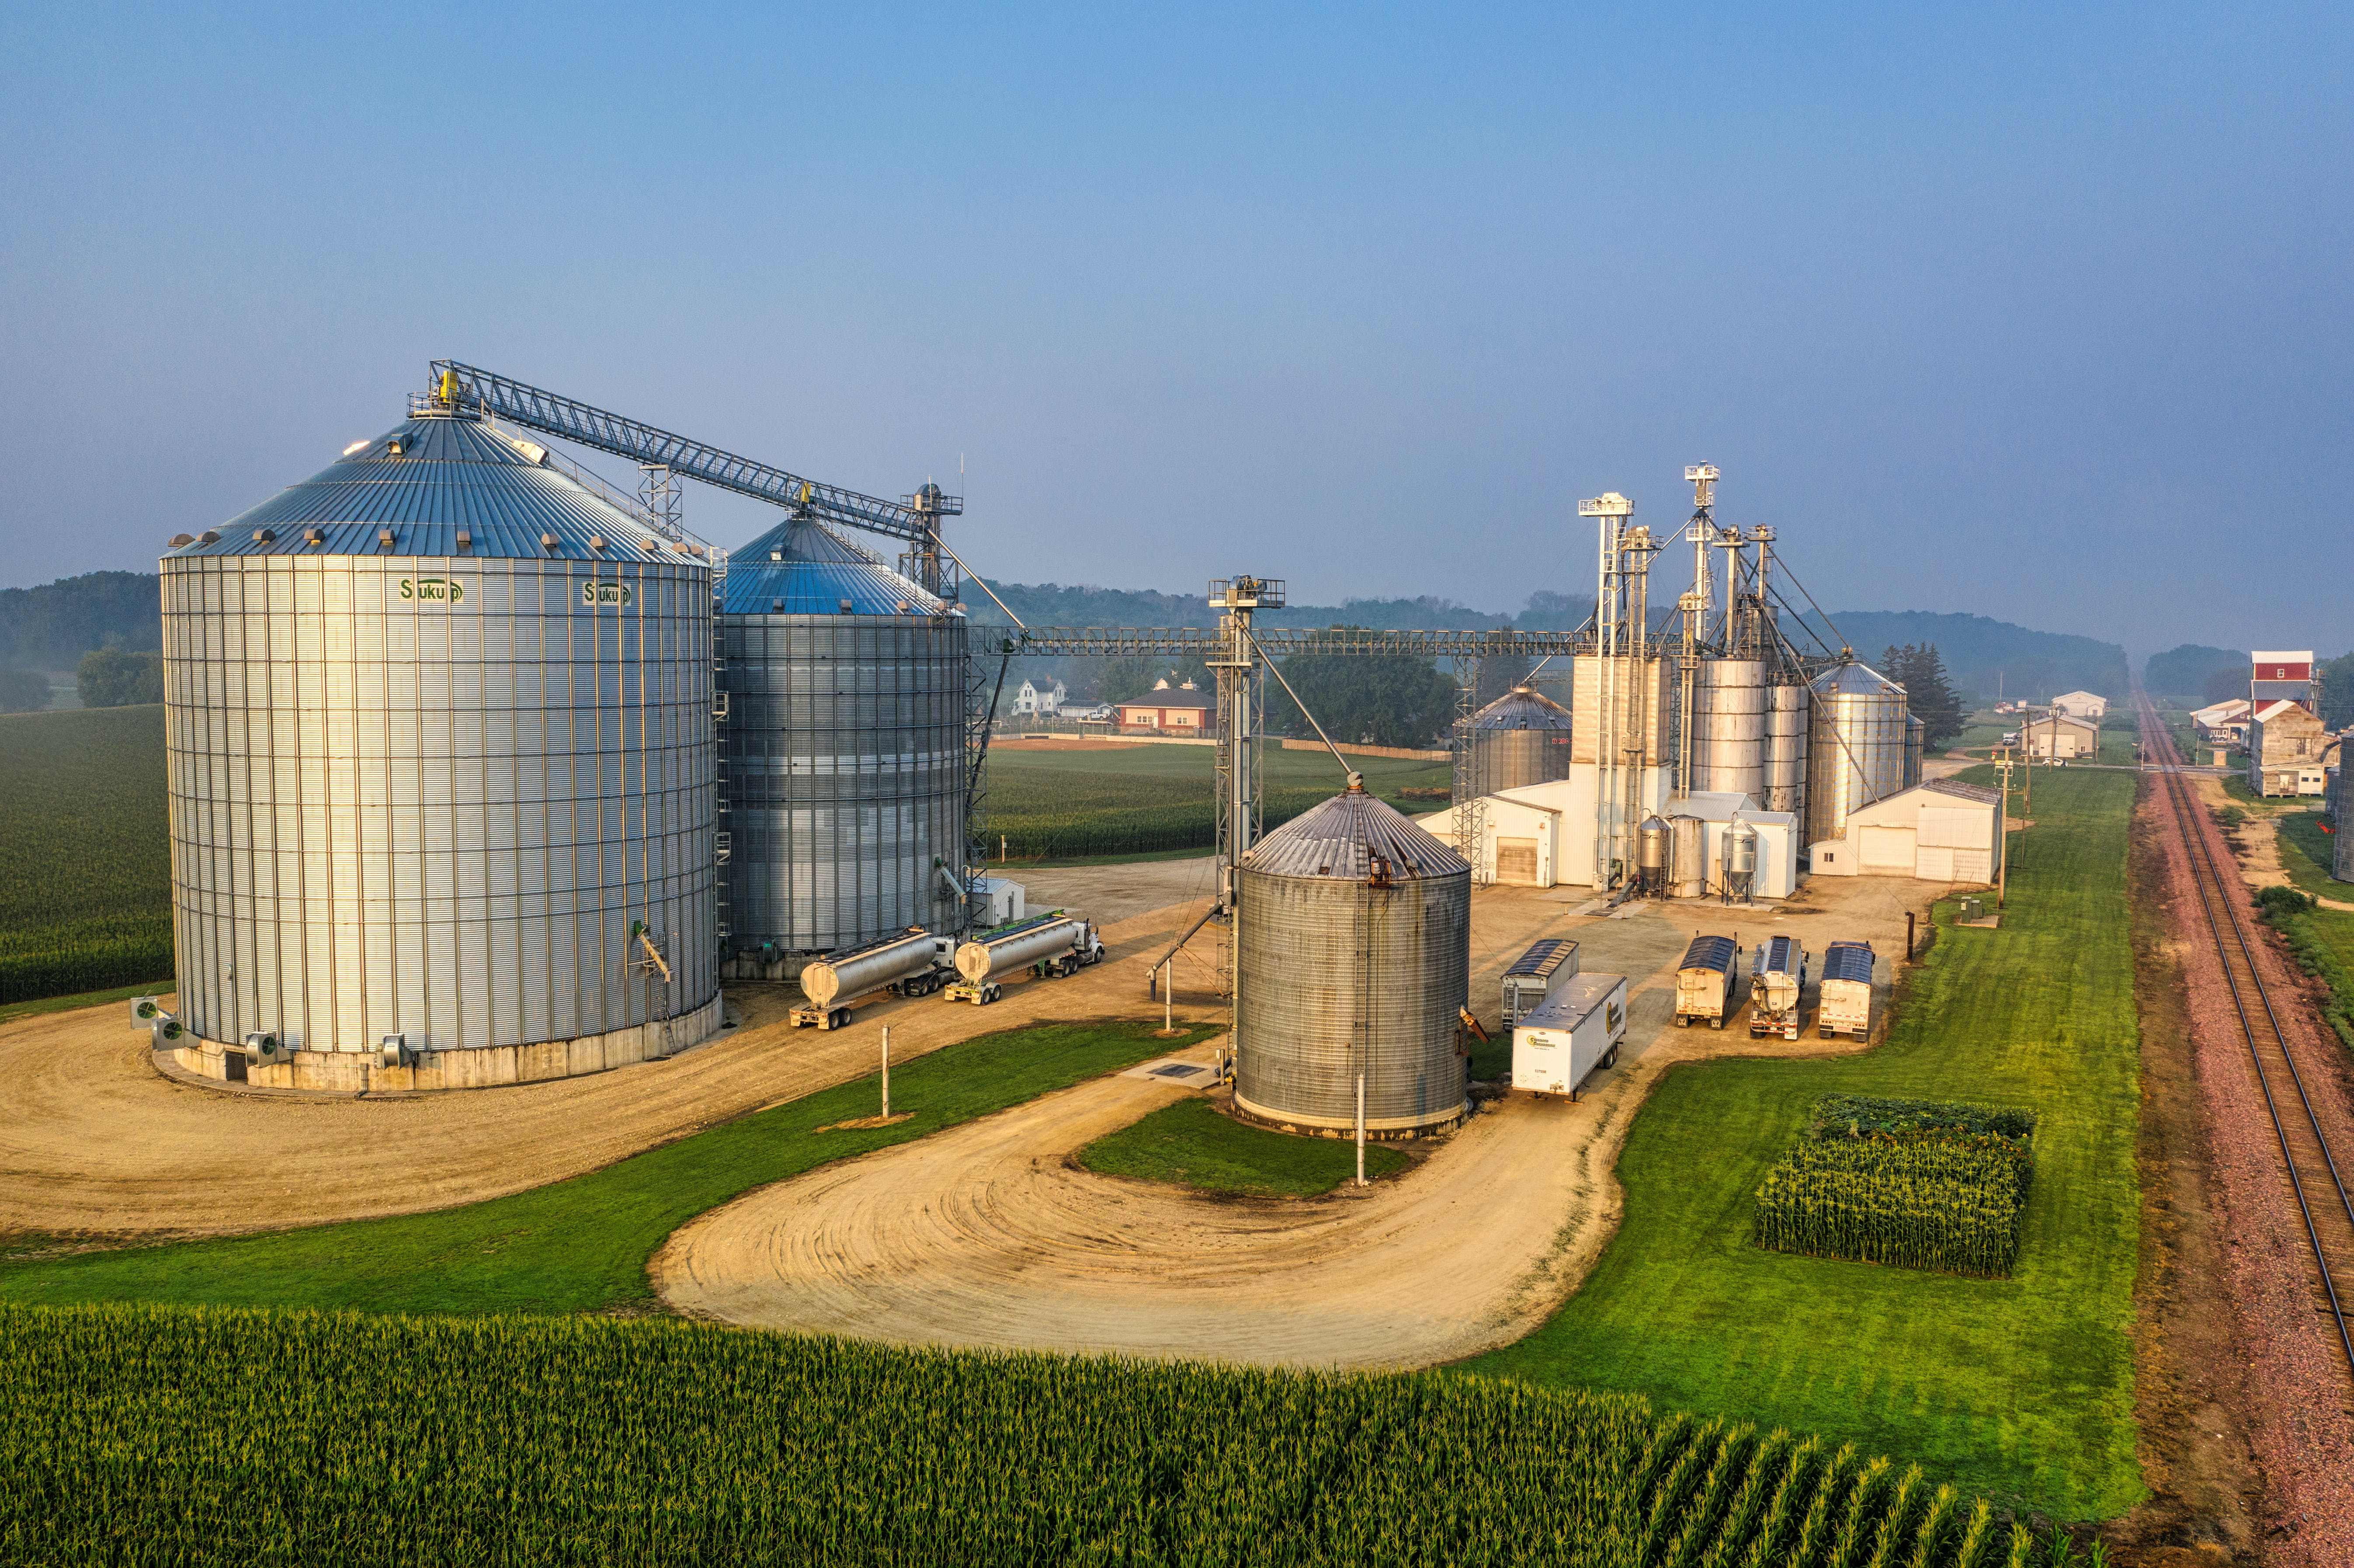
\includegraphics[width=.5\textwidth]{./Figures/PlantaAcopio.jpg}
	\caption{Planta de acopio de cereales.\protect\footnotemark}
	\label{fig:planta}
\end{figure}
\footnotetext{Imagen tomada de \url{https://www.pexels.com/es-es/}}

Los silos son construcciones para almacenar granos y otros materiales a granel. Se pueden fabricar con diferentes materiales y diseños. \citep{WEBSITE:6}
%https://es.wikipedia.org/wiki/Silo

Los acopios de cereales proveen a los productores agropecuarios un espacio de almacenamiento para las semillas cosechadas. El objetivo es preservar el cereal en condiciones óptimas durante un periodo de tiempo prolongado para luego poder comercializarlo y maximizar la calidad de los productos que derivan de ellos. \citep{ARTICLE:1}

\subsection{Condiciones de almacenamiento de granos}

Para reducir las pérdidas de calidad y de inocuidad debe comprenderse que los granos tienen dos enemigos
principales: los hongos y los insectos. En consecuencia, todos los esfuerzos que se realicen durante la poscosecha deben estar claramente orientados a prevenir el desarrollo de estos organismos perjudiciales para el grano. \citep{ARTICLE:1}

Para un almacenaje seguro, evitando hongos e insectos, es necesario que dentro del silo se registre baja temperatura y humedad. 

Conocer el contenido de humedad de los granos es imprescindible para una adecuada conservación de las semillas durante la poscosecha, pues la humedad determinará en gran medida el período durante el cual el grano puede ser almacenado sin que se deteriore su calidad. Por lo tanto, conocer la humedad será fundamental para tomar la mejor decisión en cuanto a secar el grano, acondicionarlo o almacenarlo directamente.

La humedad de almacenamiento seguro es aquella que evita el desarrollo de hongos. Esta es afectada por la humedad ambiente.

El tiempo de almacenamiento seguro es el período máximo que puede ser almacenado un grano a determinadas condiciones de humedad y temperatura, sin perder su calidad o propiedades.
Este es afectado por tres factores:

\begin{itemize}
\item La humedad con que es almacenado el grano, la cual favorece fundamentalmente el desarrollo de los hongos.
\item La temperatura. Cuanto mayor es, más rápido es el deterioro y favorece la propagación a los insectos.
\item El porcentaje de grano dañado mecánicamente. Este es más susceptible al ataque de hongos y de insectos.
\end{itemize}

Como se puede observar en la figura \ref{fig:tempHum}, la forma óptima de conservar los cereales es mantener baja temperatura y humedad.

\begin{figure}[htbp]
	\centering
	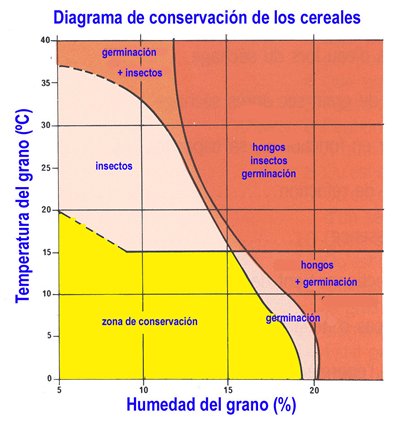
\includegraphics[width=.5\textwidth]{./Figures/DiagramaDeConservacionGranos.png}
	\caption{Diagrama conservación de los cereales.\protect\footnotemark}
	\label{fig:tempHum}
\end{figure}
\footnotetext{Imagen tomada de \url{https://www.mapa.gob.es/es/ministerio/servicios/informacion/plataforma-de-conocimiento-para-el-medio-rural-y-pesquero/observatorio-de-tecnologias-probadas/maquinaria-agricola/secado-grano.aspx}}

Las condiciones que perjudican la calidad del grano se debe monitorear periódicamente para detectar cuanto antes potenciales inconvenientes, como la combustión espontánea, y tomar acciones preventivas evitando el deterioro de las semillas. \citep{WEBSITE:5}

%----------------------------------------------------------------------------------------
\section{Estado del arte}

Si bien existen soluciones similares, pocas se encuentran en el país, lo cual implica que los costos y mantenimiento sean elevados. 

El objetivo del trabajo es crear un prototipo de monitoreo de temperatura y humedad en una planta de acopio de cereales. Luego de ello, como mejora a futuro, se pretende migrar a una solución IoT integral donde se incluyan otros tipos de sensores que faciliten la logística y seguridad en la planta. 

En la tabla \ref{tab:peces} se observan algunas alternativas para monitoreo de parámetros en almacenamiento de cereales.

\begin{table}[h]
	\centering
	\caption[]{Soluciones existentes para monitoreo en almacenamiento de cereales}
	\begin{tabular}{l c c c}    
		\toprule
		\textbf{Empresa} 	 & \textbf{Temperatura} 		& \textbf{Humedad} & \textbf{Referencia} \\
		\midrule
		  OPI & sí	& sí  & \citep{WEBSITE:4}\\		
		Avann Technologies	 & sí	& sí & \citep{WEBSITE:3}\\
		Measure Instruments	 & sí	& no & \citep{WEBSITE:1} \\
            Tornum	 & sí	& sí  & \citep{WEBSITE:2}\\
		\bottomrule
		\hline
	\end{tabular}
	\label{tab:peces}
\end{table}

En resumen, se encuentran soluciones comerciales que permiten el monitoreo de temperatura y humedad. Sin embargo, el objetivo de este trabajo es lograr consolidar los conocimientos adquiridos en la especialidad y generar una solución incremental que permita llegar a la automatización total de una planta de acopio de cereales con un costo accesible. 

%----------------------------------------------------------------------------------------
\section{Motivación}
Una empresa o cooperativa dedicada al almacenamiento de granos tiene uno o más depósitos distribuidos y para controlar el estado de almacenamiento de sus productos necesita enviar operarios a las diferentes plantas. Dada esta situación, se implementó un sistema de monitoreo IoT para optimizar tiempos y costos.

Al comenzar a buscar posibles temas para este trabajo, surgió el contacto con un posible cliente que necesita una solución integral de IoT para su planta de acopio, por este motivo se implementa un prototipo que luego irá evolucionando e integrando soluciones a diferentes problemas. 

%----------------------------------------------------------------------------------------
\section{Alcance y objetivos}

El propósito de este trabajo fue implementar el prototipo de un sistema de monitoreo para plantas de acopio de cereales, con el objetivo de reafirmar los conocimientos adquiridos en la especialización de internet de las cosas y poder implementarlo a futuro en campo. 

Esta implementación será la base de futuros desarrollos donde se planifica integrar diferentes tipos de sensores y adaptar el proyecto a las necesidades de algunos clientes.  

El alcance del trabajo incluyó:
\begin{itemize}
\item Un prototipo funcional.
\item Un nodo que simula datos obtenidos y los transmite a la nube.
\item Selección del protocolo para transmisión de datos.
\item Desarrollo / selección de \textit{backend} del sistema que procesa y almacena los datos recibidos.
\item Presentación de datos.
\end{itemize}

El presente trabajo no incluye:
\begin{itemize}
    \item La puesta en marcha del producto en las instalaciones de una planta de almacenamiento.
    \item La lectura de datos en sensores reales desde los nodos.
\end{itemize}

%----------------------------------------------------------------------------------------


